%!TEX program = xelatex
\documentclass{article}
\usepackage[a5paper,hmargin=17mm,tmargin=12mm,bmargin=12mm]{geometry}

\usepackage{ifxetex}
\ifxetex
 \usepackage{fontspec}
 \setmainfont[Scale=1.1]{Arno Pro}
 \setmonofont[Scale=.95]{Consolas}
 \usepackage{unicode-math}              %% пакет для загрузки шрифтов математического режима 
 \setmathfont{[latinmodern-math.otf]}
 \setmathfont[range=\mathit/{latin,Latin}]{Arno Pro Italic}
 \setmathfont[range=up]{Arno Pro}
\else
 \usepackage[utf8]{inputenc}
\fi
\usepackage[russian]{babel}
\usepackage{enumitem, minted, pdfpages}

\newcommand{\answerbox}[1][1.7cm]{\par\begin{tabular}{|p{.92\textwidth}|}
 \hline
 ~\linebreak\vskip#1\mbox{}
 \\
 \hline
\end{tabular}}

\begin{document}

\pagestyle{empty}
\abovedisplayskip=0pt

\subsection*{1. Простые линейные программы \hfill В1}

Не надо писать \texttt{\#include}, \texttt{\#define} и \texttt{int main()}, \\нужна только ВНУТРЕННОСТЬ функции \texttt{main()}! \\Все данные вводить в том порядке, в каком они появляются в условии.

\begin{enumerate}[left=0pt .. \parindent]
\item
Окружность радиуса $R$ поделили на $n$ равных дуг. Выведите длину одной дуги.
\\
\setlength\partopsep{-\topsep}
\begin{tabular}{|p{.46\textwidth}@{}|@{}p{.46\textwidth}|}
\hline
\multicolumn{2}{|c|}{ДОПИШИТЕ ОДИН ИЗ ВАРИАНТОВ:}
\\
\hline
 \begin{minted}{cpp}
 int R, n;
 scanf("%d %d", &R, &n);
 
 printf( 
 \end{minted}
&
 \begin{minted}{cpp}
 int R, n;
 cin >> R >> n;

 cout << 
 \end{minted}
\\
\hline
\end{tabular}
\item
Ввести радиус $R$ и вывести объем шара радиуса $R$ и площадь круга радиуса $R$ (объем шара равен $\frac{4}{3}\pi R^3$).
\answerbox
\item
Около окружности радиуса $R$ описан квадрат. Выведите \hfill\smash{\raisebox{-2.6em}
{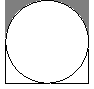
\includegraphics{pic1.pdf}}}\\
площадь заштрихованной части.\\[1mm]
\answerbox
\item
Ввести трехзначное натуральное число, вывести сумму его цифр.
\answerbox
\item
Ввести действительное число $x$, вывести значение $2x^4-x^3+5x^2-3x+4$, используя не более 4 умножений и не более 4 сложений/вычитаний.
\answerbox
\item
Ввести выражение из трех символов: цифра, знак \texttt{'*'}, цифра. Вывести его значение, подсчитанное как результат умножения однозначных чисел. Например, для ввода \texttt{5*8} вывести \texttt{40}.
\answerbox
\item
Ввести целые значения $x_1, y_1, x_2, y_2, x_3, y_3$, --- координаты трех точек параллелограма в порядке обхода против часовой стрелки. Вывести координаты $x_4, y_4$ четвертой вершины.
\answerbox[7cm]
\end{enumerate}

	
\end{document}\answerbox

